% LTeX: language=de-DE

\documentclass{article}

\usepackage[ngerman]{babel}
\usepackage{graphicx}
\usepackage[a4paper]{geometry}
\usepackage{float}
\usepackage{tabularx}
\usepackage{amsmath}
\usepackage{siunitx}
\usepackage{pdfpages}
\usepackage{minted}

% Default figure folder
\graphicspath{{res}}

% Paragraph spacing
\setlength{\parindent}{0cm}
\setlength{\parskip}{0.3em}

% Tabular row space
\renewcommand{\arraystretch}{1.5}
    
\begin{document}

\section{Kannlisten Aufgaben}

Im Folgenden werden die Lösungen zu den Aufgaben aus der Kannliste dargestellt (siehe Anhang, S.~\pageref{sec:Anhang}).

\subsection{Aufgaben 0 bis 5}

\begin{figure}[H]
    \centering
    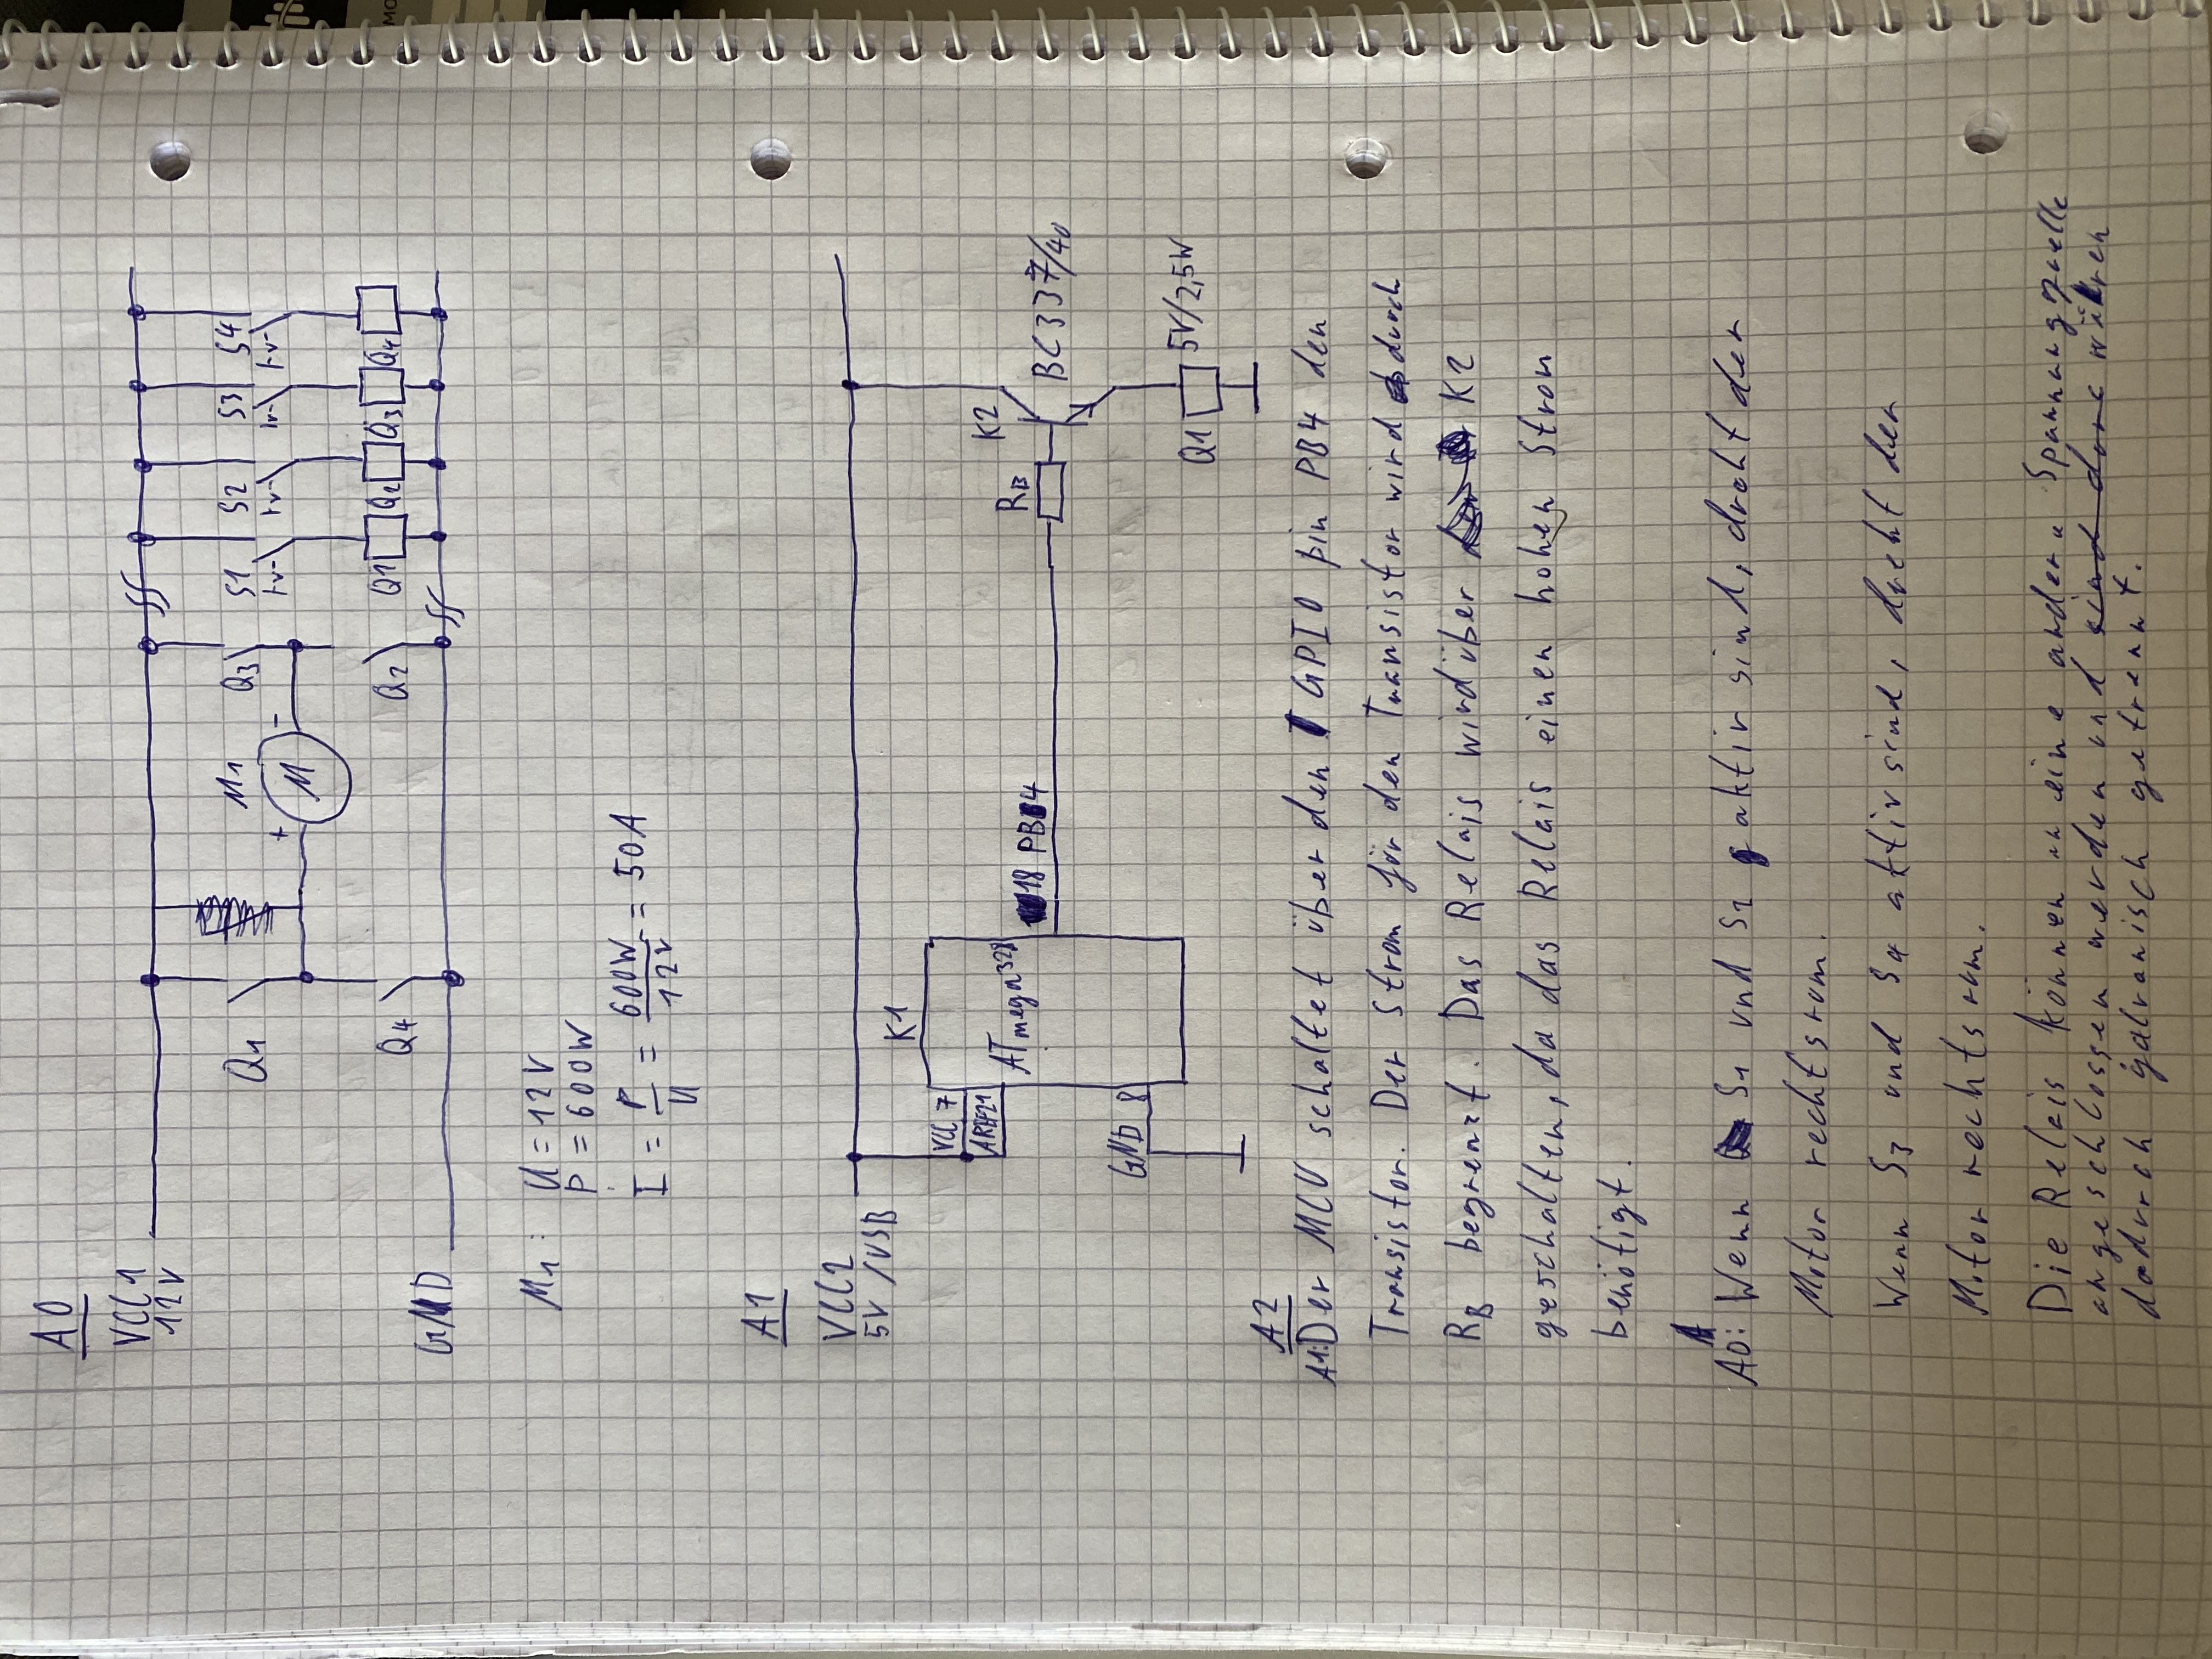
\includegraphics[angle=270, width=0.85\linewidth]{A0_to_A2.jpg}
    \caption{Aufgaben 0 bis 2}
\end{figure}

\clearpage
\begin{figure}
    \centering
    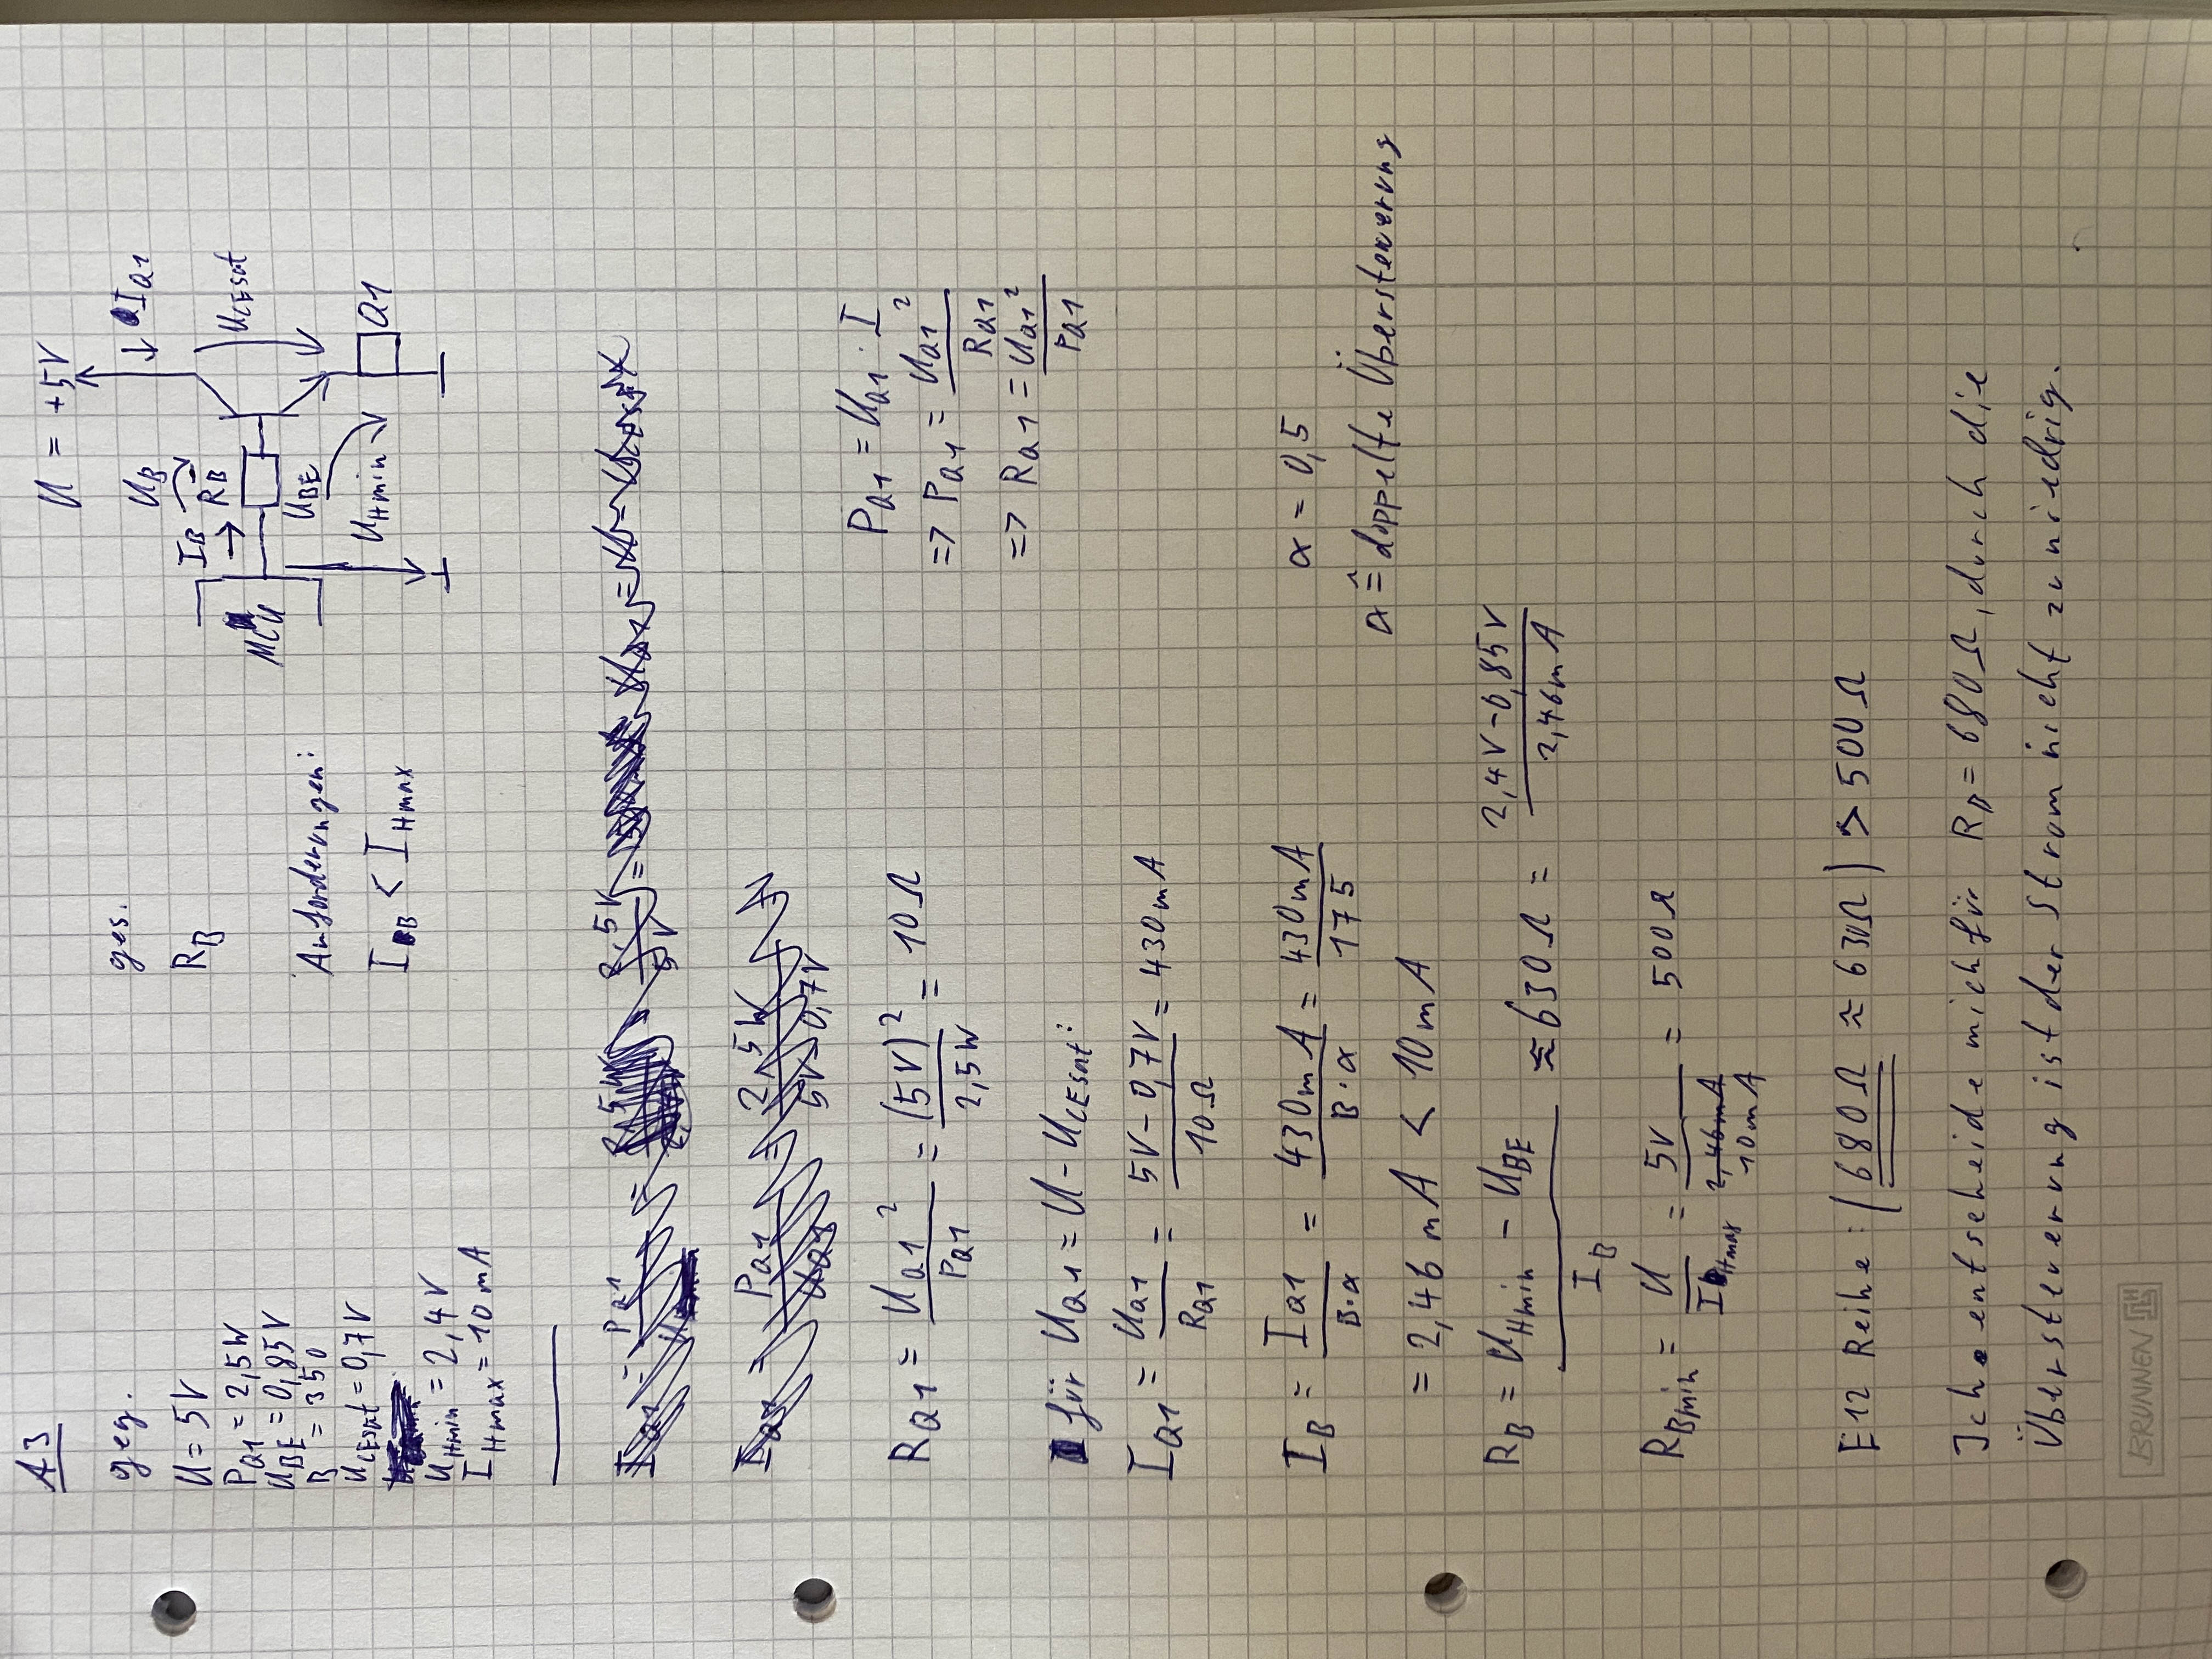
\includegraphics[angle=270, width=\linewidth]{A3.jpg}
    \caption{Aufgabe 3}
\end{figure}

\clearpage
\begin{figure}
    \centering
    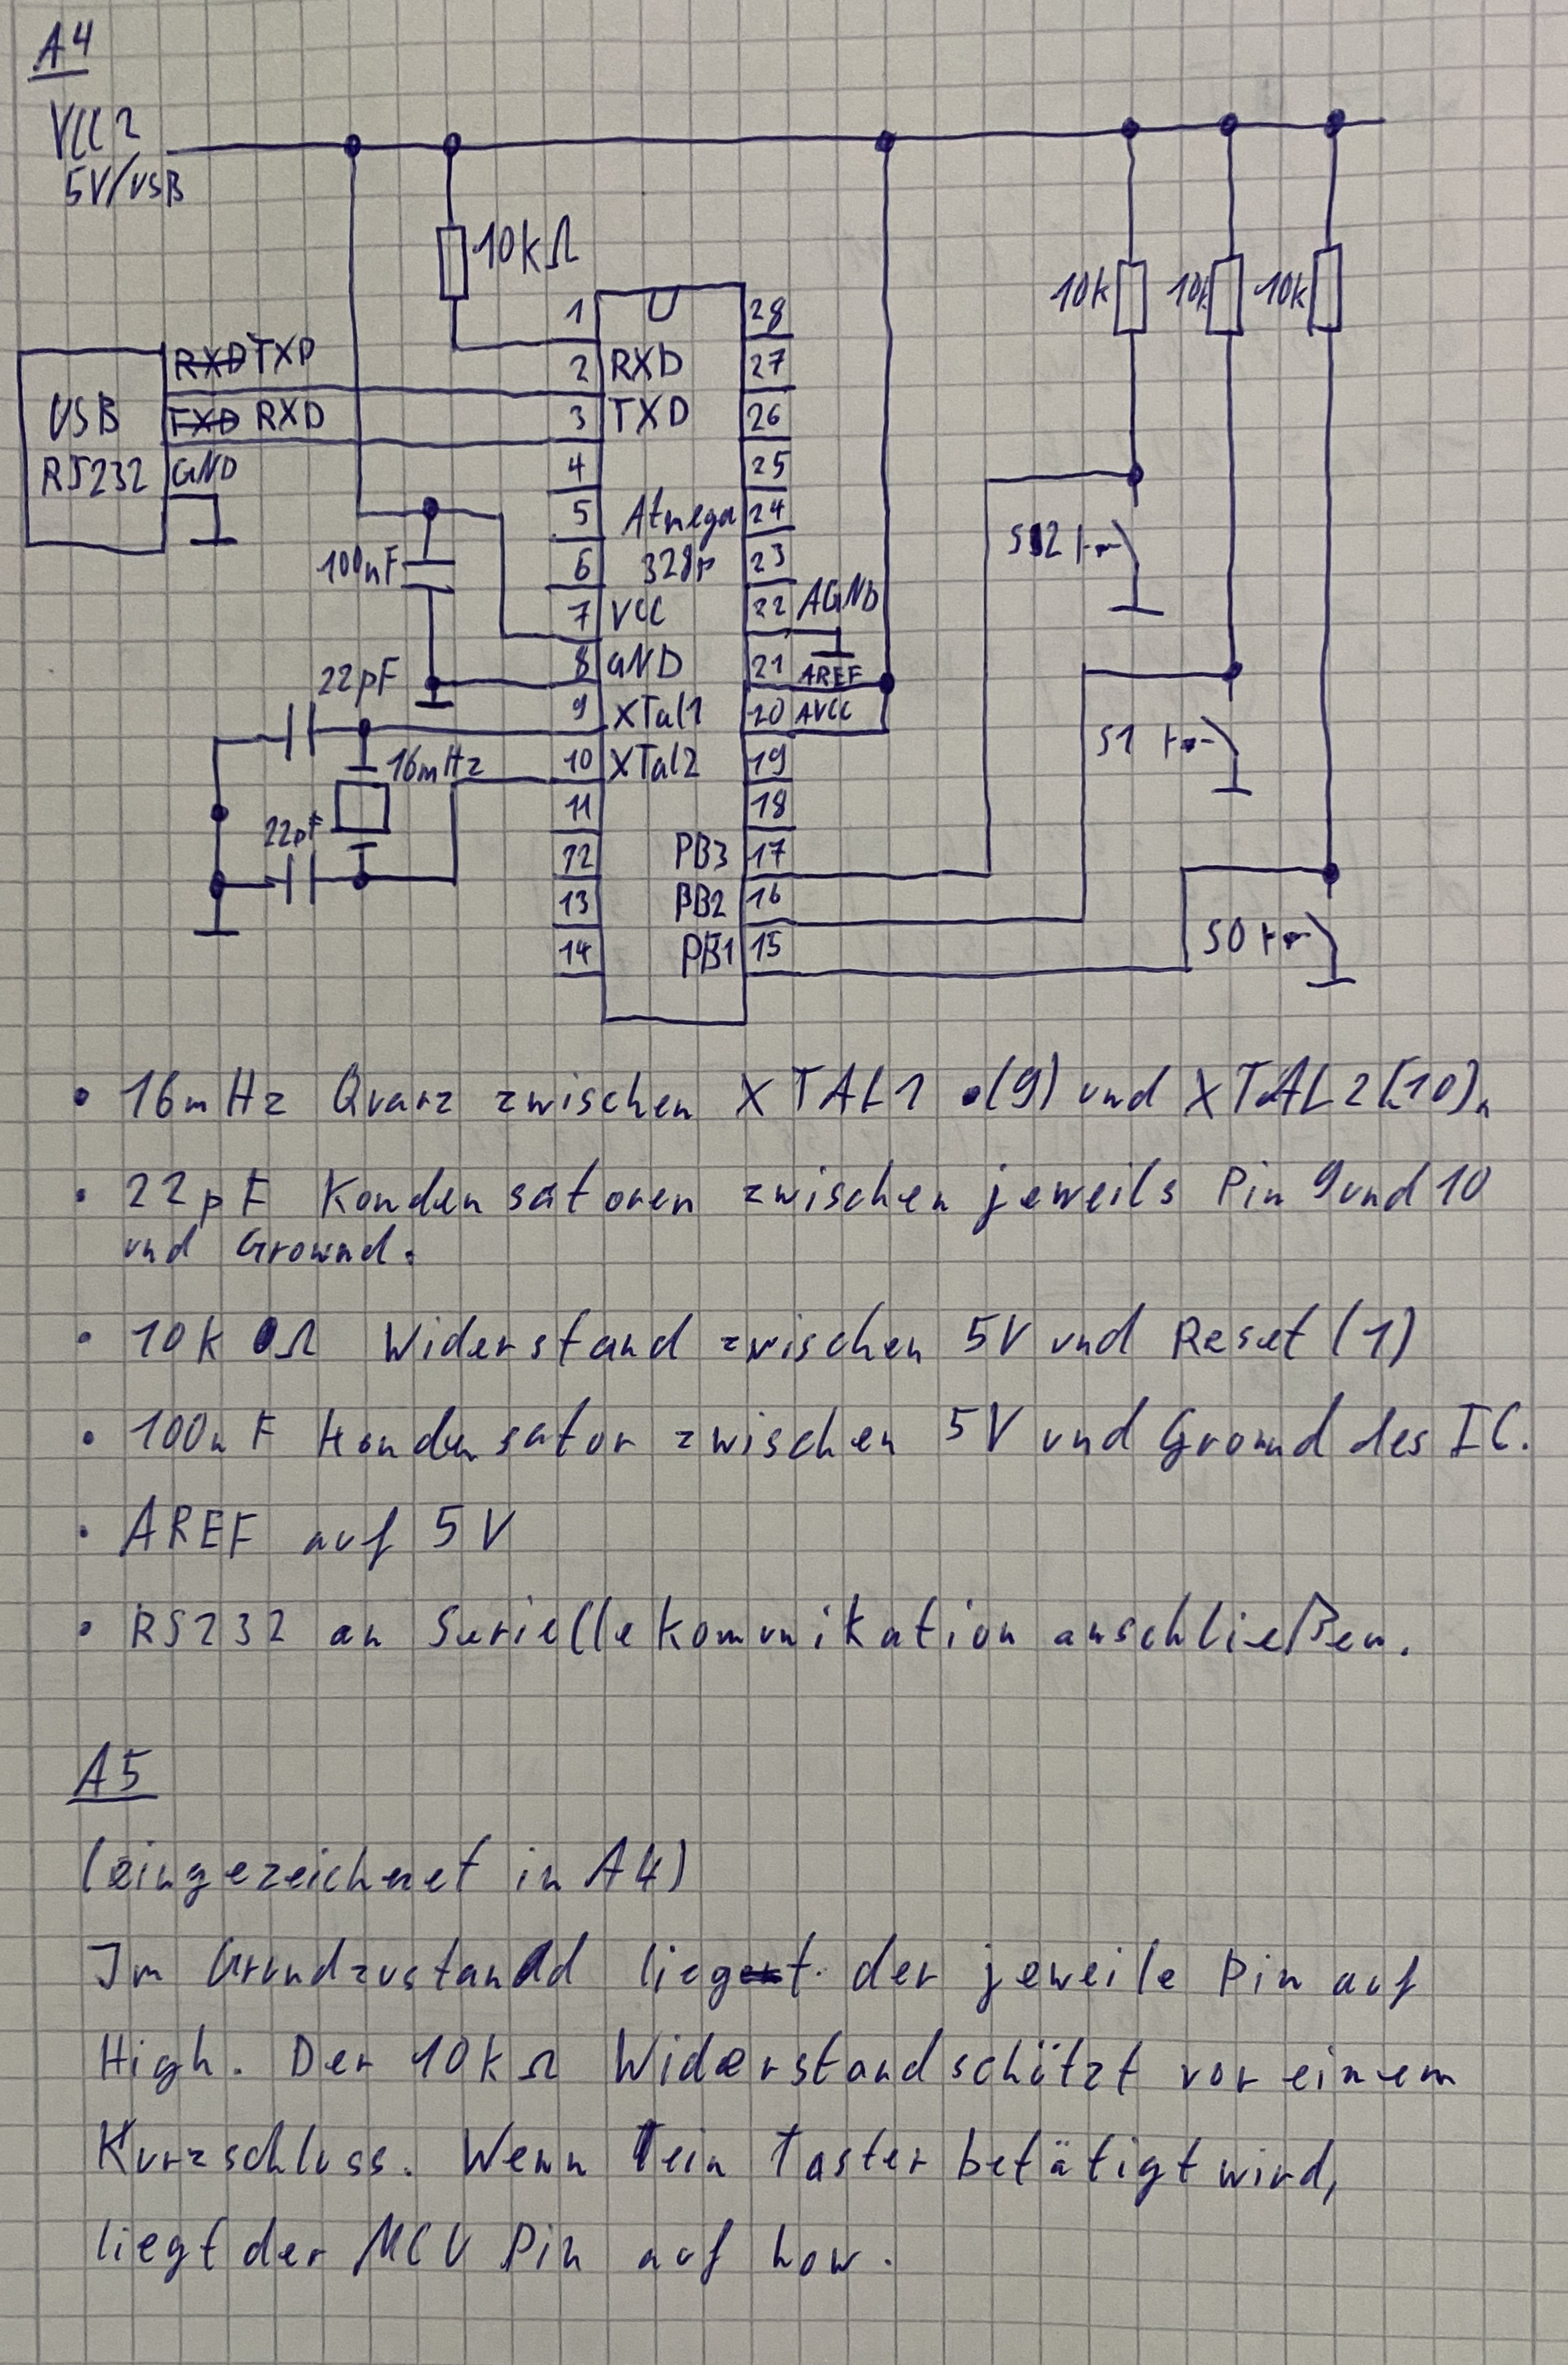
\includegraphics[width=0.85\linewidth]{A4_to_A5.jpg}
    \caption{Aufgabe 4 und 5}
\end{figure}

\clearpage
\subsection{Aufgabe 6}

\begin{figure}
    \centering
    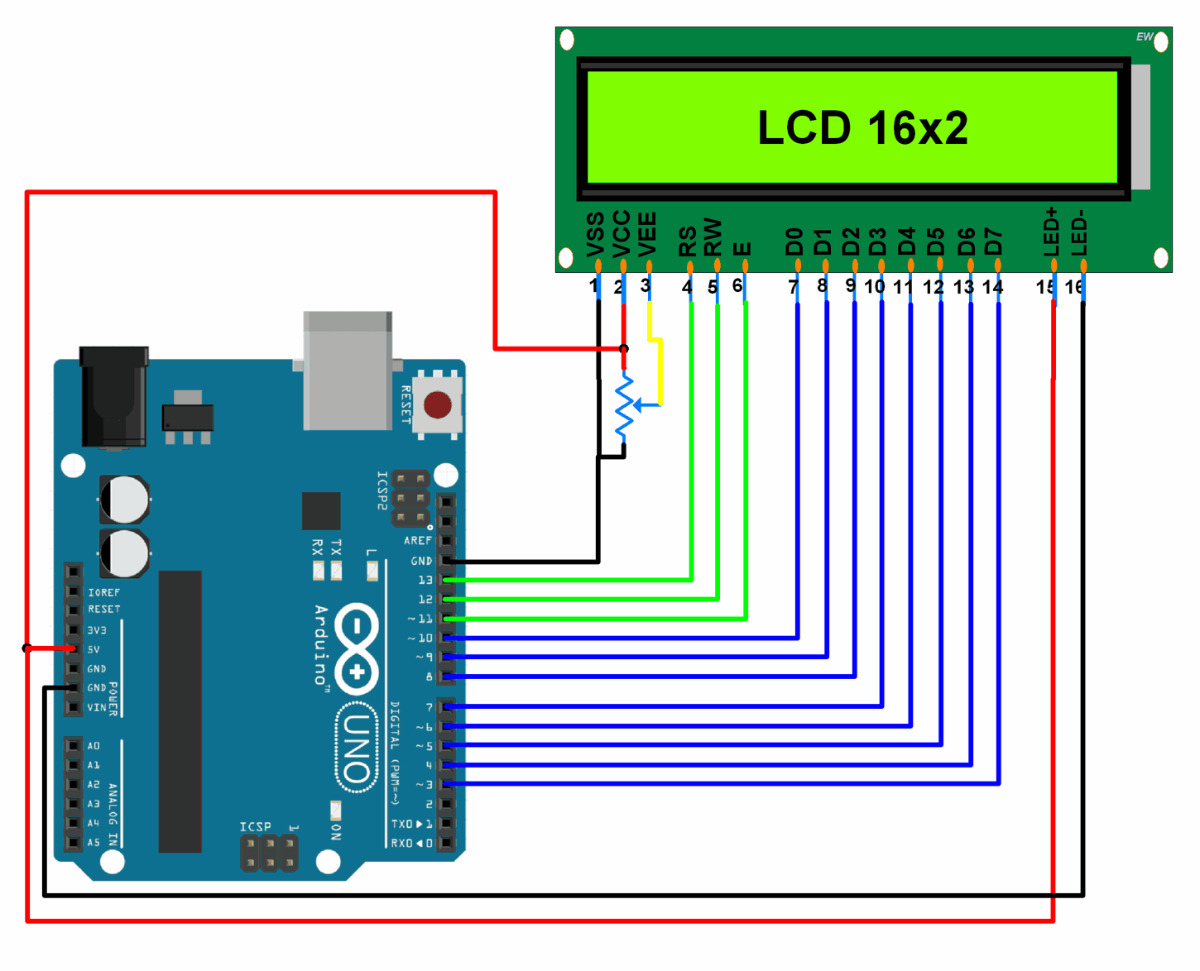
\includegraphics[width=0.75\linewidth]{LCD_Arduino_Schaltplan.jpg}
    \caption{Schaltplan um LCD (mit HD44780) an Arduino anzuschließen}
    \label{fig:lcd_arduino}
\end{figure}

In Abbildung~\ref{fig:lcd_arduino} wie man ein LCD an einen Arduino anschließen kann.
Die folgenden Pinbeschreibungen wurden aus dem Datenblatt des HD44780 entnommen.

\vspace{0.4cm}
\begin{tabularx}{\linewidth}{p{1.3cm} p{1.7cm}  X}
    \textbf{Pin} & \textbf{MCU Pin} & \textbf{Funktionen der Ausgänge des HD44780} \\
    \hline
    VSS & GND & niedriges Spannungspotential \\
    VCC & \SI{5}{\volt} & positive Spannung für das LCD und den HD44780 \\
    VEE & $[\SI{0}{\volt}; \SI{5}{\volt}]$ & Kontrast -- stellt ein wie stark sich die Kristalle drehen. \\
    RS & PB5 & 0: Instruction 1: Data register \\
    $\text{R/}\overline{\text{W}}$ & \SI{5}{\volt} & In diesem Fall wird nur geschrieben. \\
    E & PB3 & Enable -- an ihm wird das Taktsignal angelegt. \\
    D0 - D2 & PB2 - PB0 & 8 Bit Dateneingang \\
    D3 - D7 & PD7 - PD3 & 8 Bit Dateneingang \\
    LED+ & \SI{5}{\volt} & Zuständig für die Spannungsversorgung der LEDs. 
    Dabei ist darauf zu achten, dass ein Vorwiderstand in dem LCD Modul vorhanden ist. \\
    LED- & GND & Hier muss das niedrige Spannungspotential angelegt werden. \\
\end{tabularx}

\clearpage
\subsection{Aufgabe 7}

\begin{figure}[H]
    \centering
    \includegraphics[width=0.75\linewidth]{A7.jpg}
    \caption{Schaltplan um LCD (mit HD44780) an Arduino anzuschließen}
\end{figure}

\clearpage
\subsection{Allgemeiner Code}
Code der für alle Aufgaben von 8 bis 14 gilt:

\inputminted[linenos]{c++}{res/code/global.c}

\clearpage
\subsection{Aufgabe 8}
\begin{figure}[H]
    \centering
    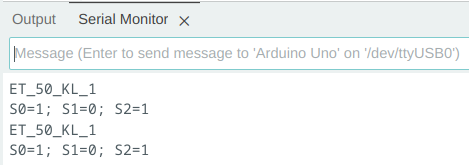
\includegraphics[width=0.75\linewidth]{ET_50_KL_01.png}
    \caption{UART-Ausgabe von ET\_50\_KL\_01}
\end{figure}
\inputminted[linenos]{c++}{res/code/ET_50_KL_01.c}

\clearpage
\subsection{Aufgabe 9}
\begin{figure}[H]
    \centering
    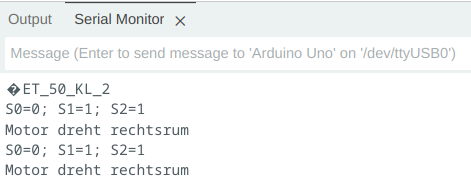
\includegraphics[width=0.75\linewidth]{ET_50_KL_02.png}
    \caption{UART-Ausgabe von ET\_50\_KL\_02}
\end{figure}
\inputminted[linenos]{c++}{res/code/ET_50_KL_02.c}

\clearpage
\subsection{Aufgabe 10}
\begin{figure}[H]
    \centering
    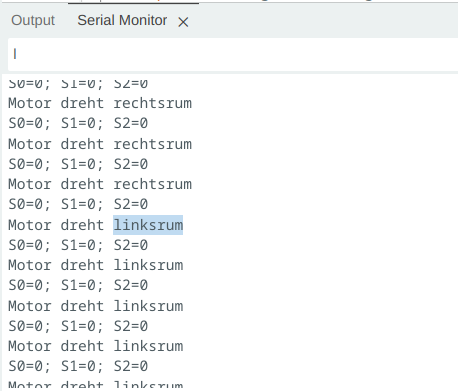
\includegraphics[width=0.75\linewidth]{ET_50_KL_03.png}
    \caption{UART-Ausgabe von ET\_50\_KL\_03}
\end{figure}
\inputminted[linenos]{c++}{res/code/ET_50_KL_03.c}

\clearpage
\subsection{Aufgabe 11}
\begin{figure}[H]
    \centering
    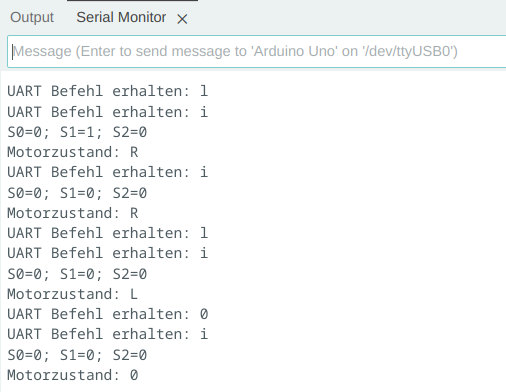
\includegraphics[width=0.75\linewidth]{ET_50_KL_04.png}
    \caption{UART-Ausgabe von ET\_50\_KL\_04}
\end{figure}
\inputminted[linenos]{c++}{res/code/ET_50_KL_04.c}

\clearpage
\subsection{Aufgabe 12}
\begin{figure}[H]
    \centering
    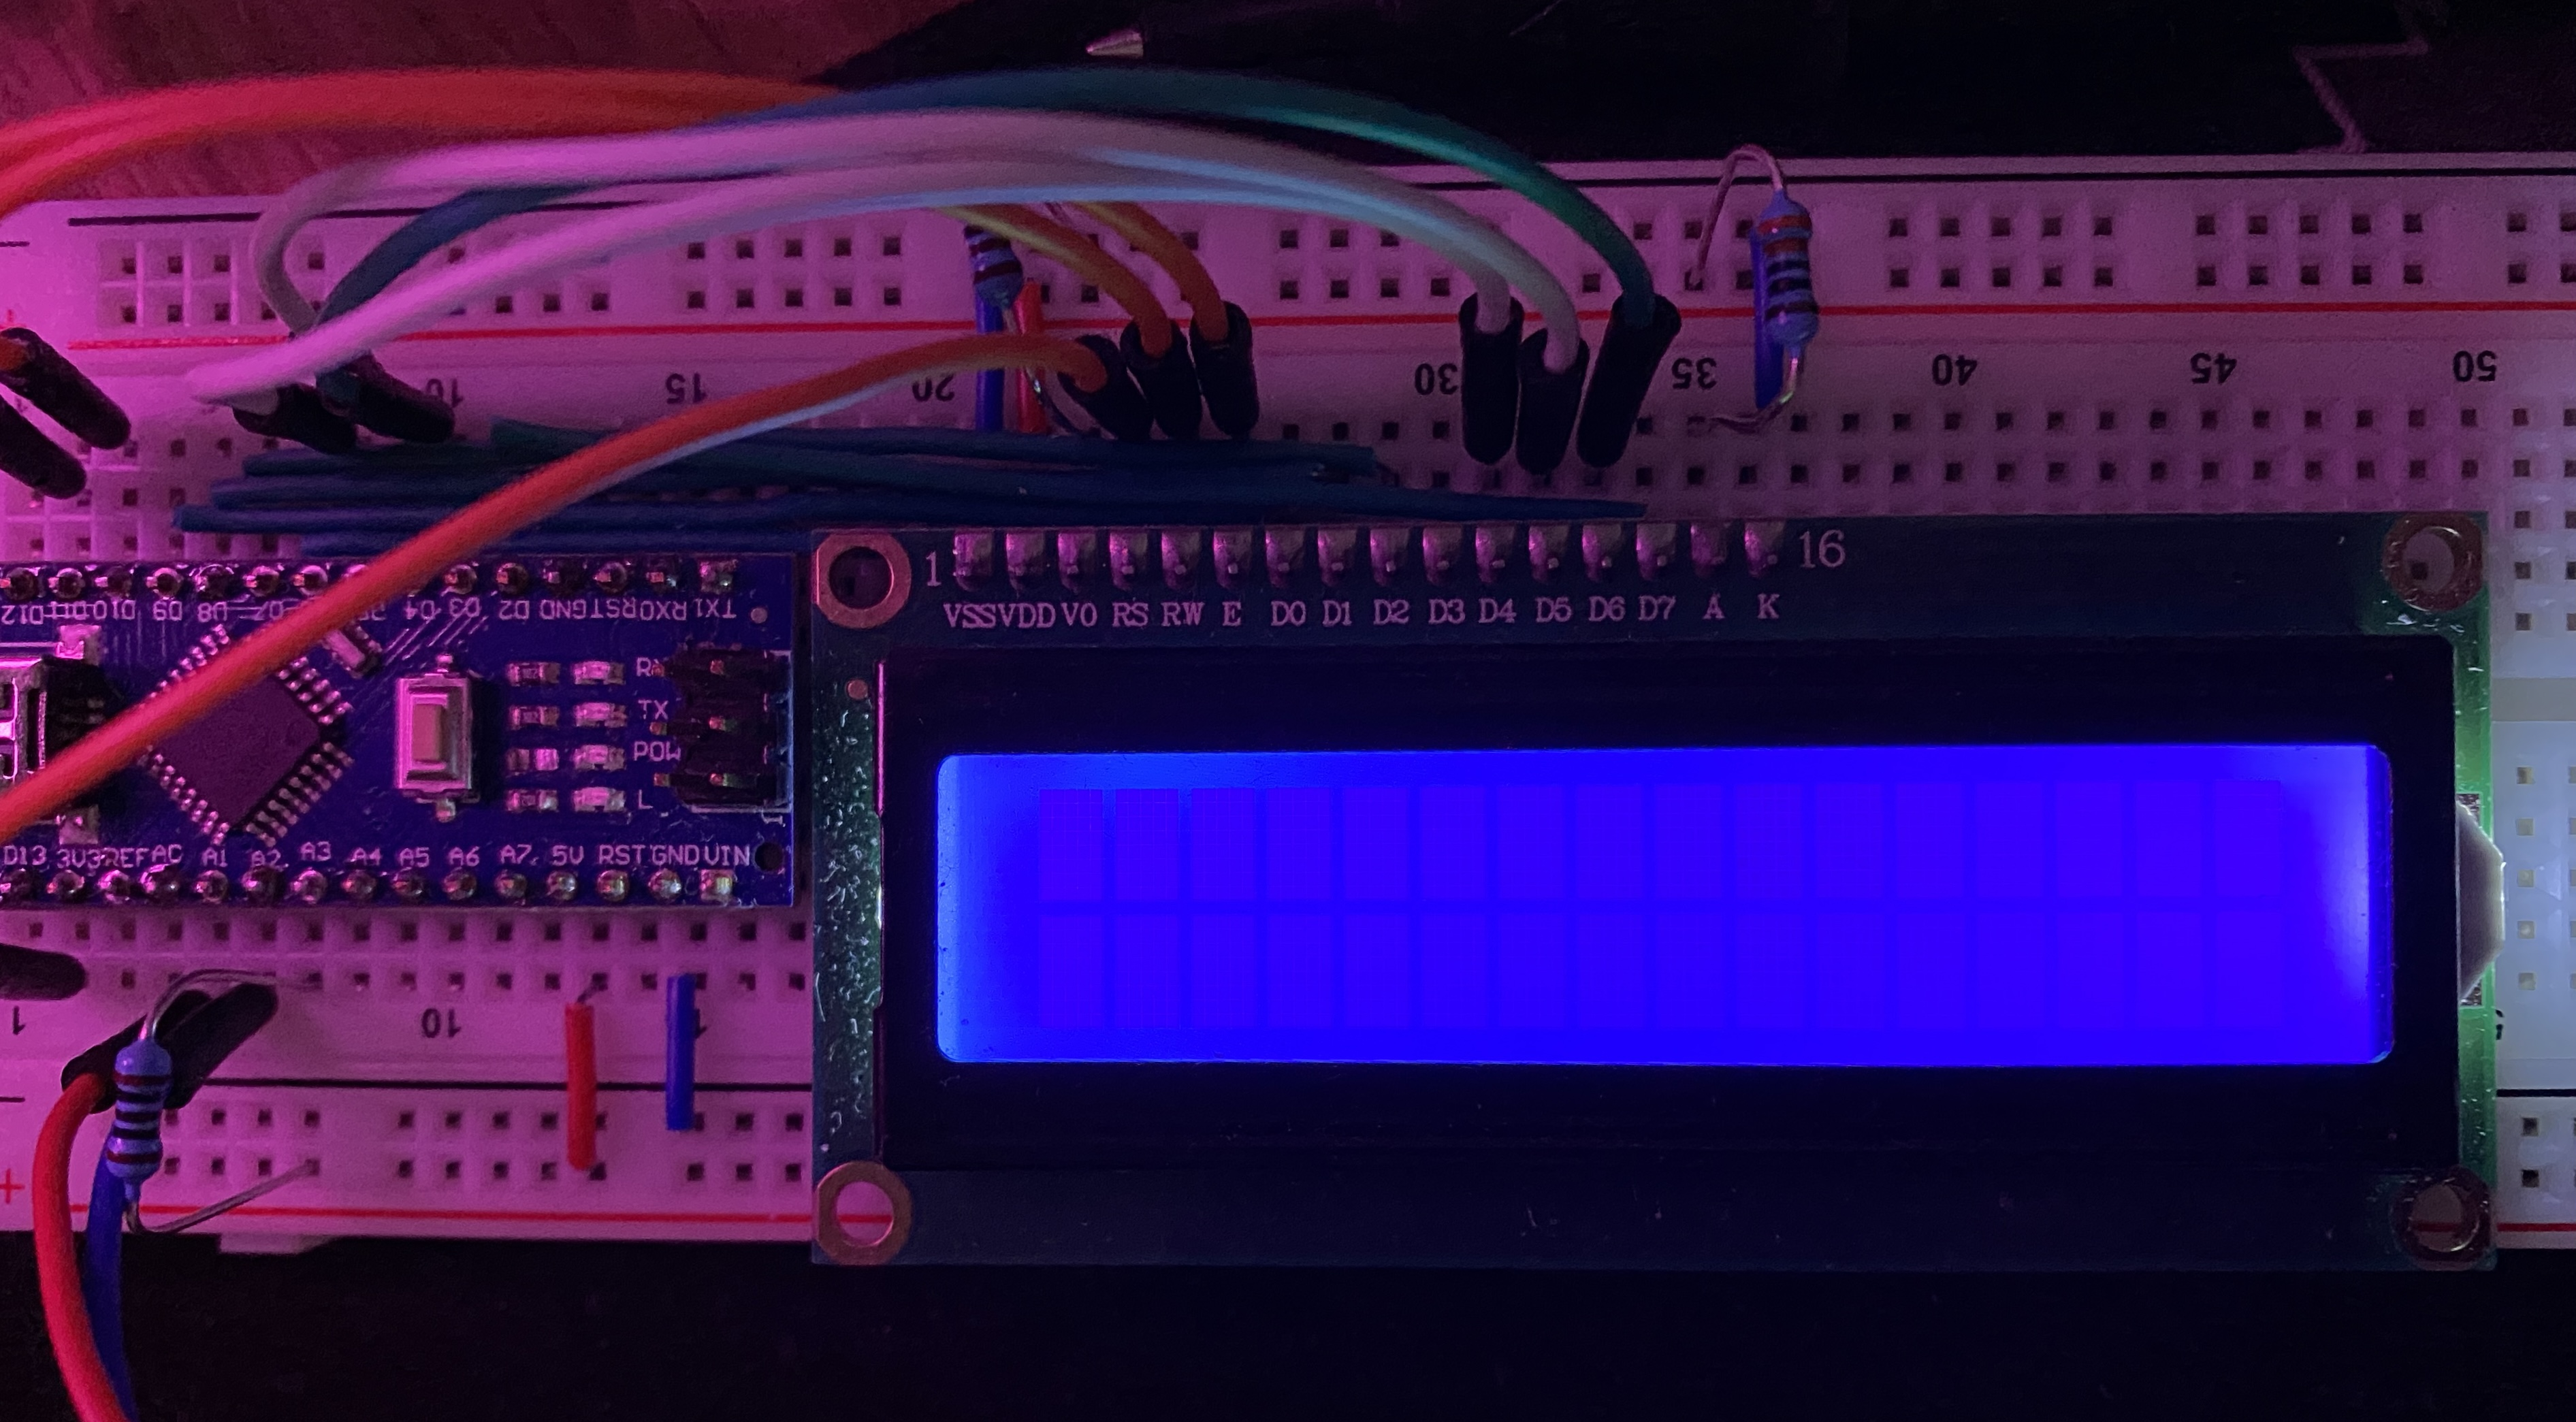
\includegraphics[width=0.75\linewidth]{ET_50_KL_05.jpg}
    \caption{Initialisiertes LCD von ET\_50\_KL\_05}
\end{figure}
\inputminted[linenos]{c++}{res/code/ET_50_KL_05.c}

\clearpage
\subsection{Aufgabe 13}
\begin{figure}[H]
    \centering
    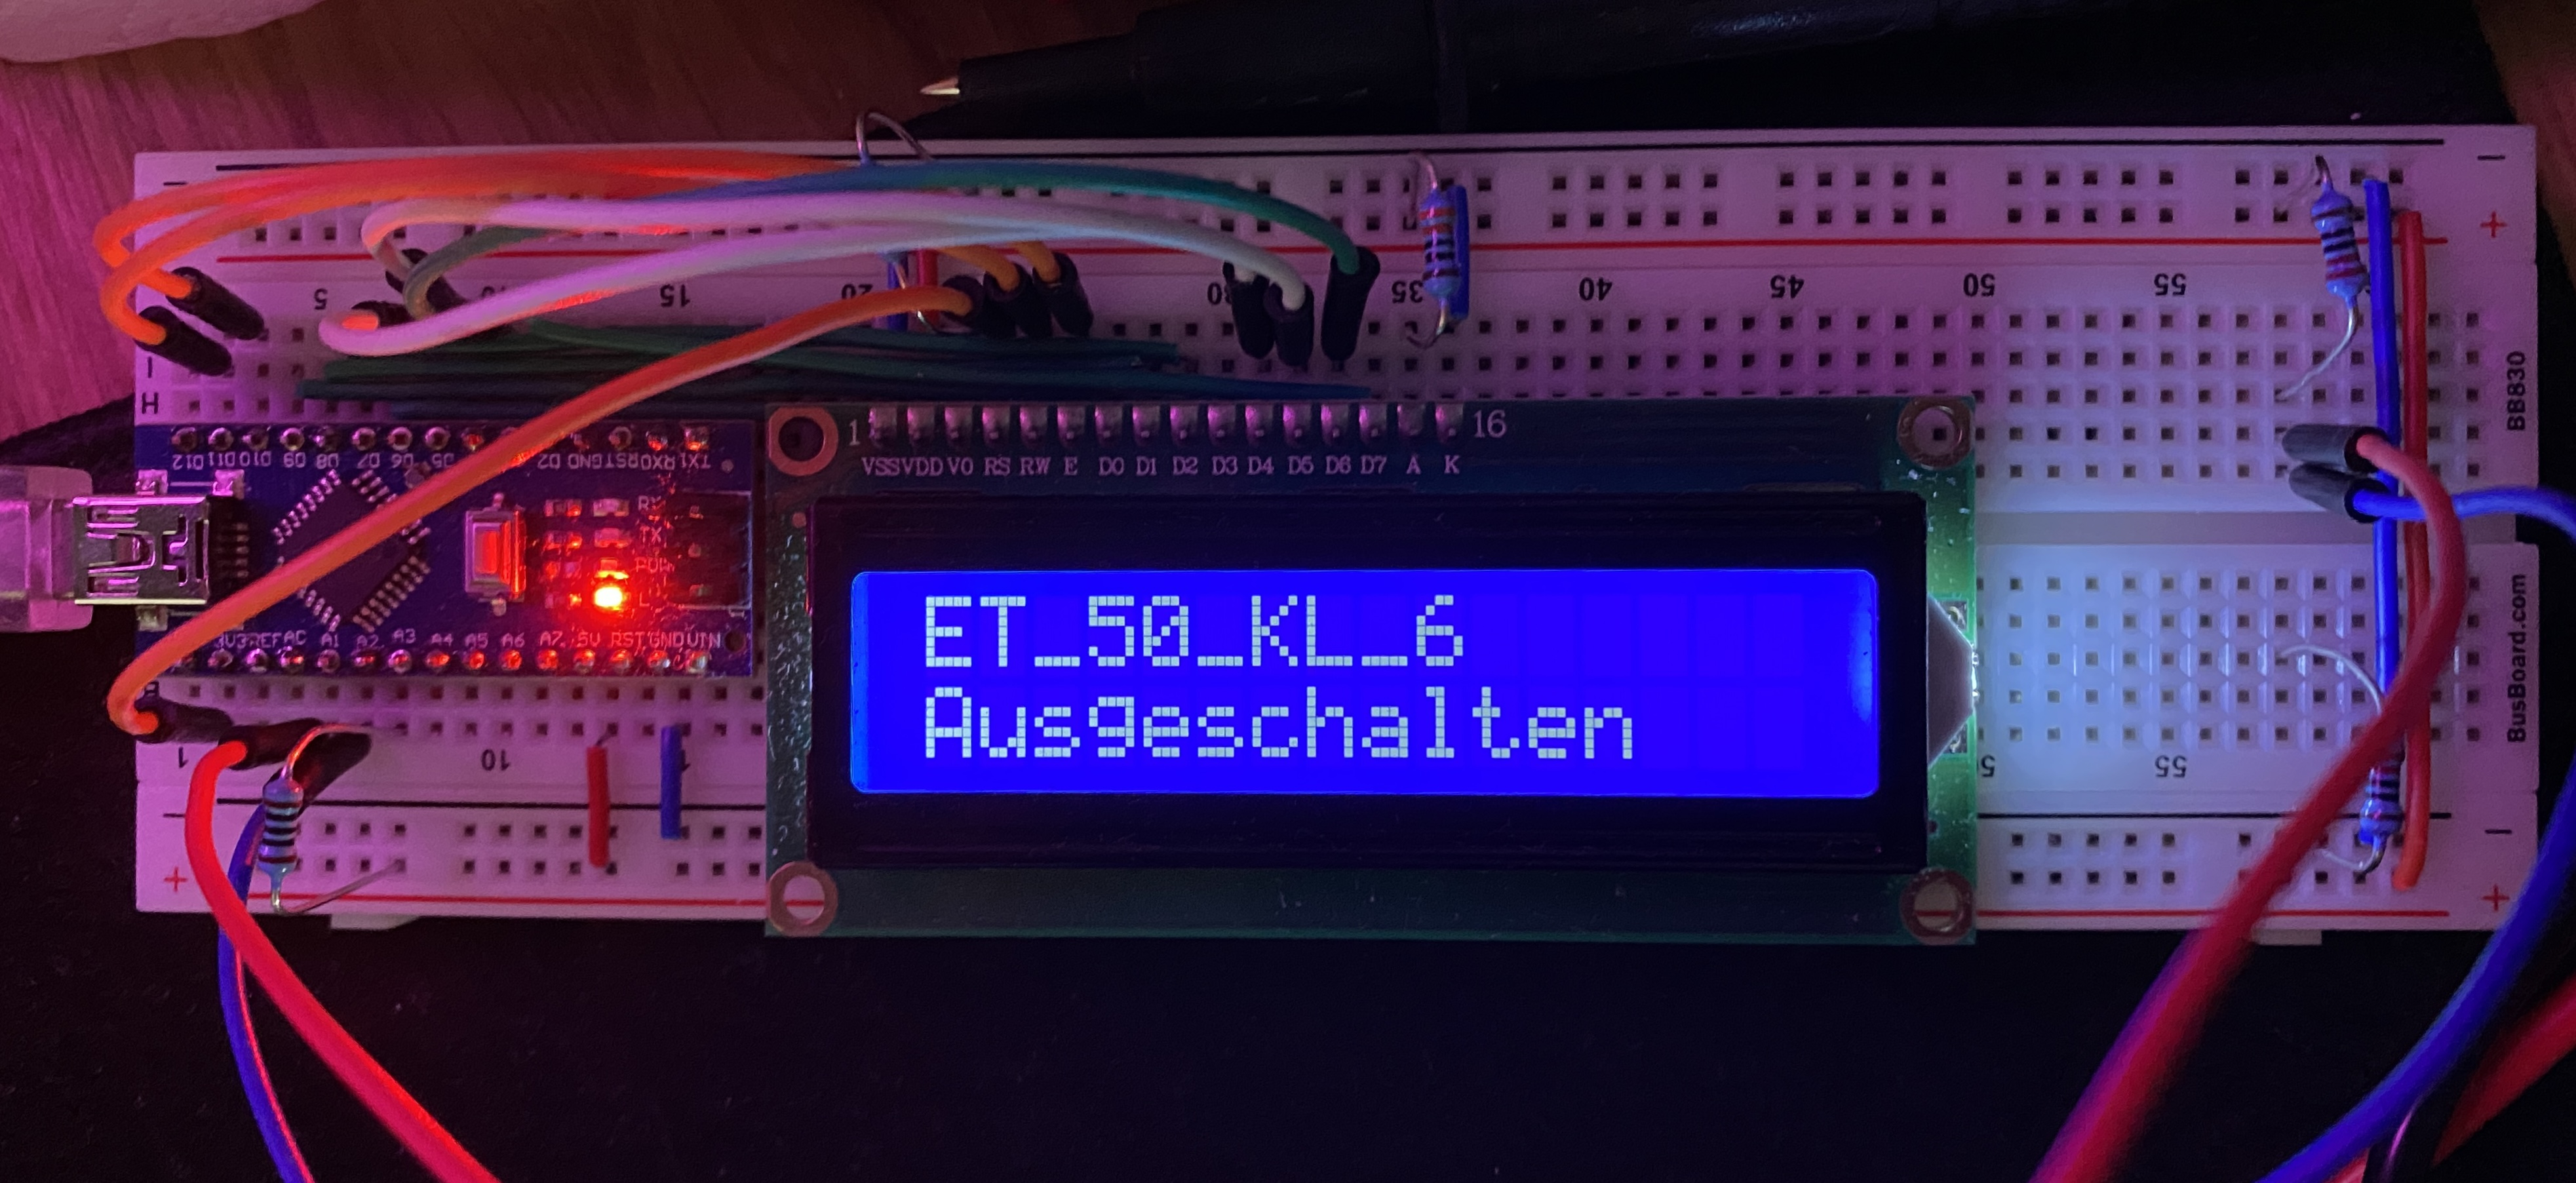
\includegraphics[width=0.75\linewidth]{ET_50_KL_06.jpg}
    \caption{Version und Motorzustand auf LCD von ET\_50\_KL\_06}
\end{figure}
\inputminted[linenos]{c++}{res/code/ET_50_KL_06.c}

\clearpage
\subsection{Aufgabe 14}
\inputminted[linenos]{c++}{res/code/global.c}
\inputminted[linenos]{c++}{res/code/ET_50_KL_07.c}

\clearpage
\label{sec:Anhang}
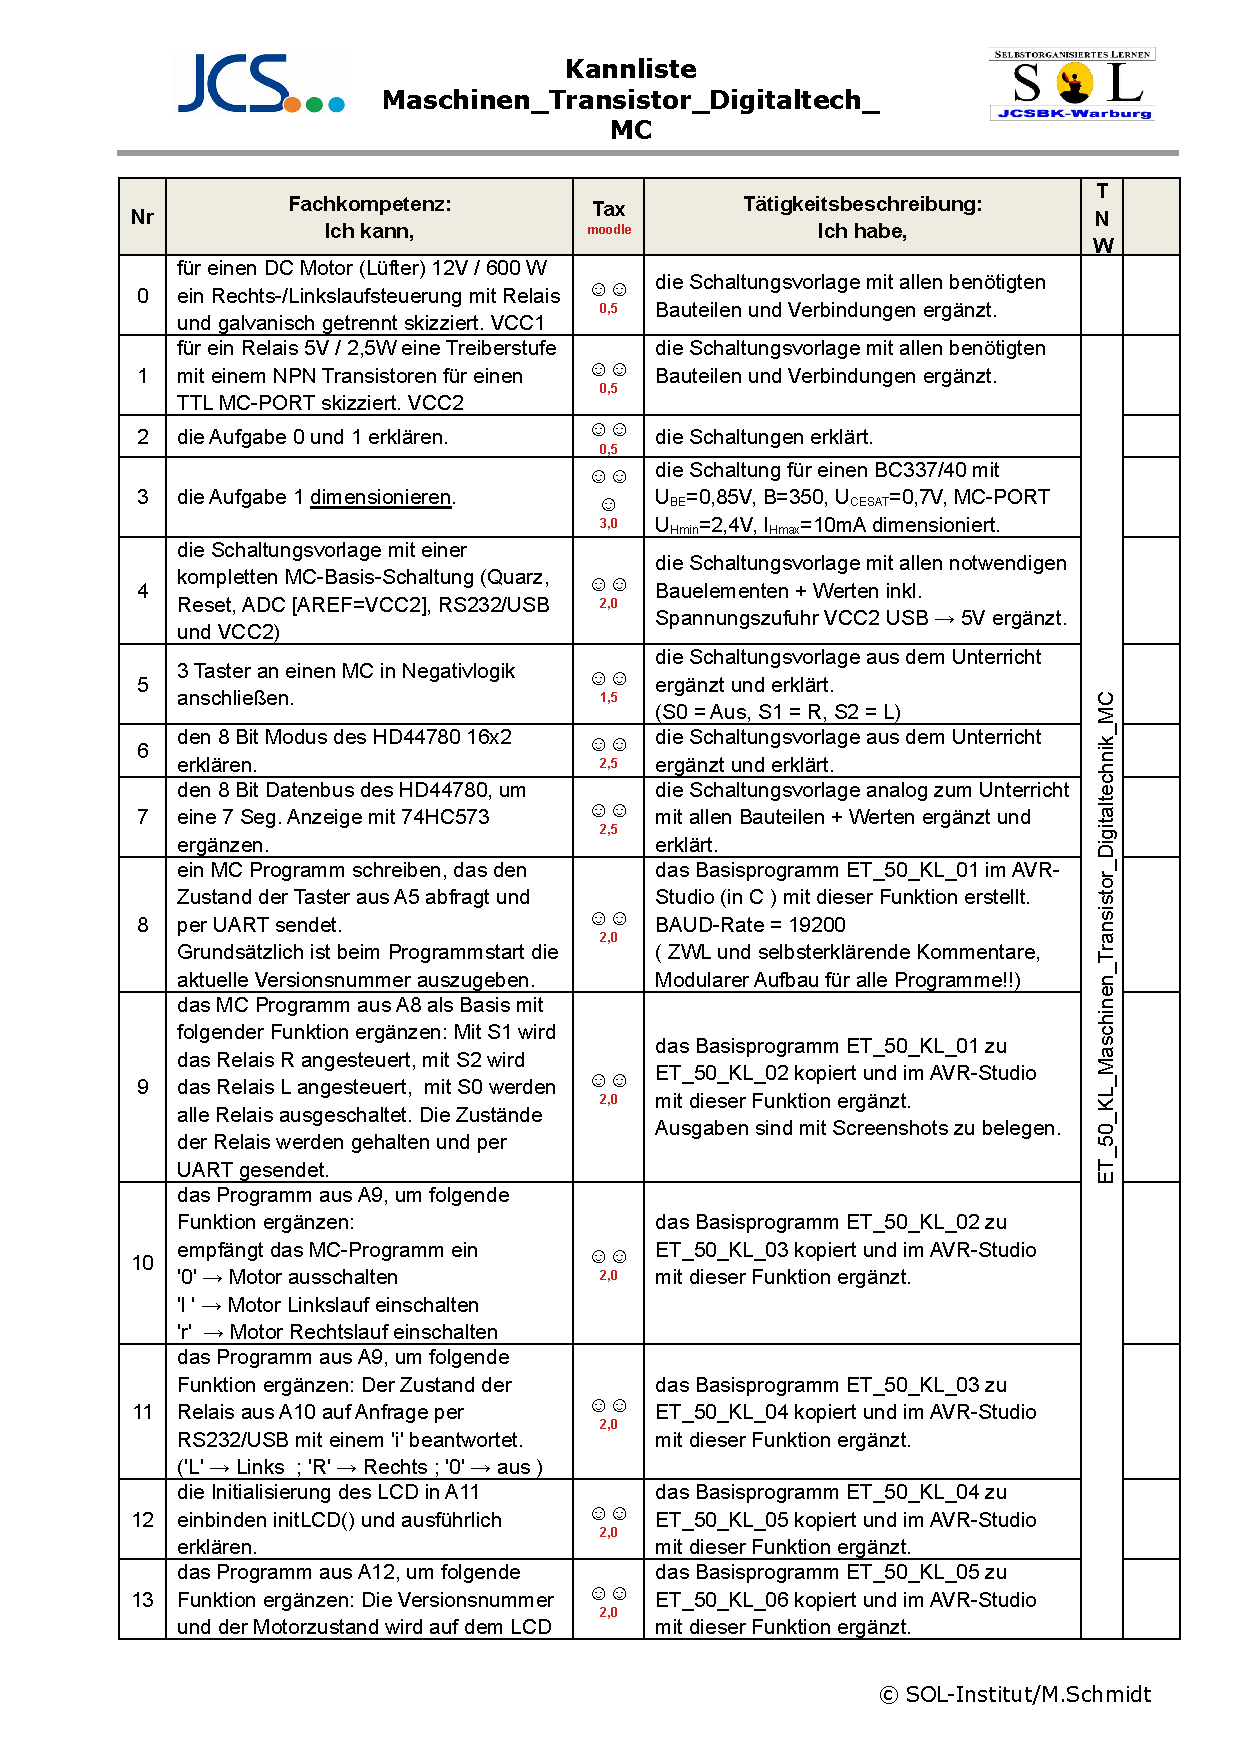
\includepdf[pages=-]{res/Kannliste.pdf}

\end{document}
